\documentclass[10.5pt]{config}
% 本实验报告采用 署名-相同方式共享 4.0 国际许可协议 (CC BY-SA 4.0)
\usepackage{multirow}
\usepackage{wrapfig}
\usepackage{setspace}
\usepackage{titlesec}
\usepackage{ctex}
\usepackage{graphicx} % 用于插入图片
\usepackage{float}    % 用于控制图片位置
\usepackage{makecell}
\usepackage{tikz}
\usetikzlibrary{arrows.meta}

\titleformat{\subsubsection}[block]  % 设置为块级标题（自动换行）
{\normalfont\bfseries}{\thesubsubsection}{1em}{} 
\titlespacing*{\subsubsection}{1.5em}{3.25ex}{1.5ex}  % 调整缩进：左缩进2em
\setstretch{1.5}

% --- 请在这里填写您的个人信息 ---
\major{} % 专业
\name{}
\partner{} % 签名栏
\stuid{}
\date{}
\lab{}
\grades{}
\course{电工电子学实验}
\instructor{} % 指导老师
\exptype{基础实验} % 实验类型
\expname{单相交流电特性及功率因数提高} % 实验名字


\begin{document}

\makeheader % 首页头部

\section{实验目的和要求}

\begin{enumerate}[label=\arabic*., leftmargin=2em]
    \item 了解电感性电路提高功率因数的方法和意义。
    \item 学会使用交流仪表（电压表、电流表、功率表）。
    \item 掌握用交流仪表测量交流电路电压、电流和功率的方法。
\end{enumerate}

\section{实验内容和原理}


\subsection{实验原理}

交流电路中常用的无源电路器件有电阻、电感和电容，利用交流电压表、交流电流表、功率表测量有关的电压、电流和功率，可以算得被测电路的有关参数。交流电路中的负载通常有电阻性负载，如白炽灯、电阻加热器等，也有电感性负载，如电动机、变压器、电磁线圈等。电磁线圈通常带有铁芯，在交流工况下铁芯会产生一定的损耗，因此一个具有铁芯的线圈在交流工况下其等效电阻是不等于直流工况下的等效电阻的。

\subsubsection*{1. 线圈参数的测量}

将一个 $R$ 値电阻与线圈串联后接在工频交流电源上（开关 S 断开），用交流电压表和交流电流表分别测量有效値 $U$、$U_R$、$U_L$、$I$（$=I_{RL}$）。以电源电压相量 $\dot{U}$ 为参考相量，由相量关系可得：
\begin{equation*}
    \cos\varphi_{RL} = \frac{U^2 + U_R^2 - U_L^2}{2U_R U}, \quad
    \sin\varphi_{RL} = \sqrt{1 - \cos^2\varphi_{RL}}
\end{equation*}
\begin{equation*}
    X_L = \frac{U\sin\varphi_{RL}}{I_{RL}} \quad \text{或} \quad
    L = \frac{U\sin\varphi_{RL}}{\omega I_{RL}}, \quad
    R_L = \frac{U\cos\varphi_{RL} - U_R}{I_{RL}}
\end{equation*}

\subsubsection*{2. 并联电容提高功率因数}

工业上大量的设备为电感性负载，由于电感性负载存在较大的感抗，因而电路的功率因数较低。对于电感性负载，可以采用并联电容器的方法来提高电路的功率因数，从而提高电源设备的利用率，降低输电线路中的损耗。

当开关 S 闭合时，在外加正弦交流电压 $\dot{U}$ 的作用下，各支路电流的关系为
\begin{equation*}
    \dot{I} = \dot{I}_{RL} + \dot{I}_C
\end{equation*}
并联容量适当的电容 $C$ 后，电容电流 $\dot{I}_C$ 补偿了电流 $\dot{I}_{RL}$ 的部分无功分量，使得电路总电流 $\dot{I}$ 的数値减小，$\dot{U}$ 与 $\dot{I}$ 的相位差 $\varphi$ 减小，功率因数提高。但若并联电容的容量过大，总电流 $\dot{I}$ 又会增大，功率因数下降，所以与电感性电路并联的电容量要适当。

\subsubsection*{3. 功率表的使用}

交流电路所消耗的有功功率可以用功率表（也称瓦特表）来测量。功率表内部包含电流测量部件与电压测量部件。电流测量部件工作时与被测电路相串联，电压测量部件工作时与被测电路相并联。测量负载功率时，电压测量端口的“$*$”端和电流测量端口的“$*$”端连接在一起后接到电源端，读数为正表示被测电路吸收功率，读数为负表示被测电路发出功率。



\section{主要仪器设备}
\begin{enumerate}[label=\arabic*., leftmargin=2em]
    \item 实验电路板。
    \item 电工电子综合实验台。
    \item 数字式万用表。

\end{enumerate}

\section{操作方法和实验步骤}

\subsection*{1. 交流电压、电流及功率的测量}
用实验电路板上的镇流器替代线圈，白炽灯替代电阻。按图1接好实验电路，调节交流电源电压 $U$ 至 220V，测量不接电容时 $R_L$ 支路的电流 $I_{RL}$、电源电压 $U$、镇流器（线圈）两端电压 $U_L$、电阻性负载（白炽灯）两端电压 $U_R$ 及电路功率 $P$、功率因数 $\lambda$，记入表1。


\begin{figure}[H]
    \centering
    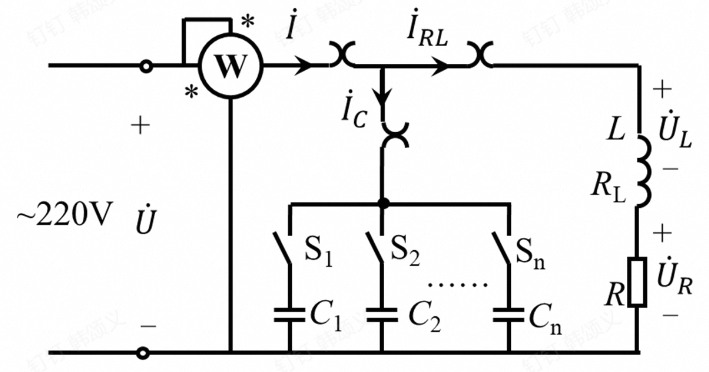
\includegraphics[width=0.5\textwidth, keepaspectratio]{figures/lianxian.png}
    \caption{电路连线}
\end{figure}

\subsection*{2. 并联电容对功率因数的影响}
测量并联不同电容量时的总电流 $I$ 和各支路电流 $I_{RL}$、$I_C$ 及电路功率 $P$、功率因数 $\lambda$，记入表2。注意并联电容 $C$ 要涵盖电路性质是感性和容性两种情况。


\section{实验数据记录和处理}
\subsection{数据记录}

% 表5.4-1 交流电压、电流及功率的测量
\begin{table}[H]
    \centering
    \small
    \begin{tabular}{|c|c|c|c|c|c|c|}
        \hline
        \multicolumn{6}{|c|}{测量値} & 计算値 \\
        \hline
        $U/\mathrm{V}$ & $U_L/\mathrm{V}$ & $U_R/\mathrm{V}$ & $I_{RL}/\mathrm{A}$ & $P/\mathrm{W}$ & $\lambda$ & $\cos\varphi_{RL}$ \\
        \hline
         226.7& 166.8&124.9 &0.245 &38.5 &0.697 & 0.698\\
        \hline
    \end{tabular}
    \caption{交流电压、电流及功率的测量}
    \label{tab:ac_measure}
\end{table}

% 表5.4-2 并联电容对功率因数的影响
\begin{table}[H]
    \centering
    \small
    \begin{tabular}{|c|c|c|c|c|c|c|c|}
        \hline
        \multirow{2}{*}{并联电容 $C/\mu\mathrm{F}$} & \multicolumn{5}{c|}{测量値} & 计算値 & \multirow{2}{*}{电路性质} \\
        \cline{2-7}
         & $I/\mathrm{A}$ & $I_C/\mathrm{A}$ & $I_{RL}/\mathrm{A}$ & $P/\mathrm{W}$ & $\lambda$ & $\cos\varphi$ & \\
        \hline
        0.5 &0.221 &0.0392 &0.246 &38.7 &0.771 &0.772 & 感性\\
        \hline
        1.0 &0.204 &0.0778 &0.245 &38.6 &0.838 & 0.837& 感性\\
        \hline
        1.5 &0.193 &0.1178 &0.245 &38.4 &0.905 &0.904 & 感性\\
        \hline
        2.0 &0.188 &0.1470 &0.244 &38.1 &0.934 &0.934 & 感性\\
        \hline
        2.5 &0.194 &0.1765 &0.244 &38.0 & 0.921& 0.920& 容性\\
        \hline
        3.0 &0.184 &0.220 &0.244 &38.0 &0.881 &0.882 &容性 \\
        \hline
        3.5 &0.204 &0.258 & 0.244&38.3 &0.799 &0.800 & 容性\\
        \hline
        4.0 & 0.225&0.294 &0.244 &38.2 &0.700 &0.700 & 容性\\
        \hline
    \end{tabular}
    \caption{并联电容对功率因数的影响}
    \label{tab:capacitor_pf}

\end{table}

根据实验数据绘制了并联电容和功率因数的曲线图

\begin{figure}[H]
    \centering
    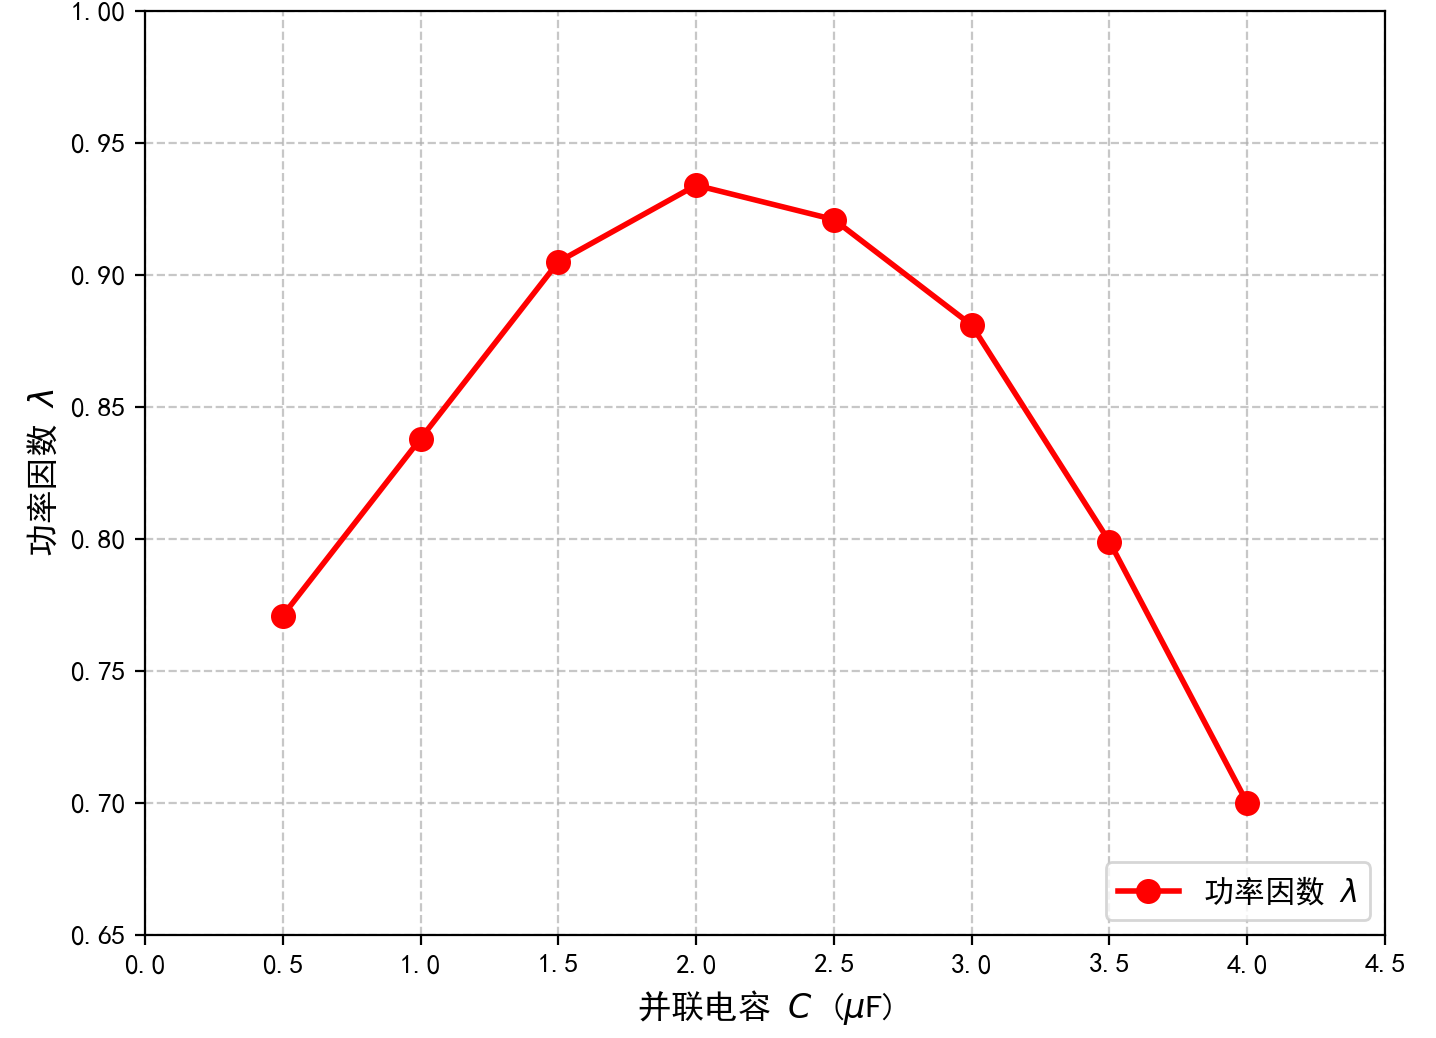
\includegraphics[width=0.5\textwidth, keepaspectratio]{figures/guanxi.png}
    \caption{并联电容和功率因数关系}
\end{figure}


\subsection{数据处理}

\subsubsection*{1. 电路参数计算}

已知我国工频交流电频率 $f = 50\text{ Hz}$，角频率 $\omega = 2\pi f \approx 314.16\text{ rad/s}$。
根据表1中的实测数据 $U = 226.7\text{ V}$，$U_L = 166.8\text{ V}$，$U_R = 124.9\text{ V}$，$I_{RL} = 0.245\text{ A}$，$P = 38.5\text{ W}$，具体计算过程如下：

\begin{itemize}[leftmargin=2em]
    \item \textbf{白炽灯电阻 $R$：}
    \begin{equation*}
        R = \frac{U_R}{I_{RL}} = \frac{124.9}{0.245} \approx 509.8 \, \Omega
    \end{equation*}

    \item \textbf{镇流器等效电阻 $R_L$：} \\
    根据有功功率公式 $P = I_{RL}^2(R + R_L)$，可得：
    \begin{equation*}
        R_L = \frac{P}{I_{RL}^2} - R = \frac{38.5}{0.245^2} - 509.8 \approx 641.4 - 509.8 = 131.6 \, \Omega
    \end{equation*}

    \item \textbf{镇流器感抗 $X_L$：} \\
    镇流器两端阻抗 $Z_L = \frac{U_L}{I_{RL}} = \frac{166.8}{0.245} \approx 680.8 \, \Omega$。由阻抗三角形关系 $Z_L^2 = R_L^2 + X_L^2$ 得：
    \begin{equation*}
        X_L = \sqrt{Z_L^2 - R_L^2} = \sqrt{680.8^2 - 131.6^2} \approx 668.0 \, \Omega
    \end{equation*}

    \item \textbf{镇流器电感 $L$：}
    \begin{equation*}
        L = \frac{X_L}{\omega} = \frac{668.0}{314.16} \approx 2.13\text{ H}
    \end{equation*}
\end{itemize}

\subsubsection*{2. 向量图绘制}

根据表1的测量数据，以电源电压 $\dot{U}$ 为参考相量（水平方向），电流 $\dot{I}$ 滞后角度 $\varphi \approx 45.8^\circ$。按比例绘制的相量图如下：

\begin{figure}[H]
    \centering
    \begin{tikzpicture}[scale=1.2, >=Stealth, thick]
        % 定义坐标和长度(按比例缩小: U~5.6, UR~3.1, UL自动闭合, I单独比例)
        \def\angle{-45.8}
        
        % 画坐标轴虚线
        \draw[dashed, gray!60] (-1,0) -- (7,0);
        \draw[dashed, gray!60] (0,-4) -- (0,2);
        
        % U (226.7V -> 长度5.67)
        \draw[->, blue] (0,0) -- (5.67,0) node[above] {$\dot{U}$ (226.7V)};
        
        % I (方向滞后45.8度, 长度单独定为3以方便观察)
        \draw[->, red] (0,0) -- ({3*cos(\angle)}, {3*sin(\angle)}) node[right] {$\dot{I}$ (0.245A)};
        
        % UR (124.9V -> 长度3.12，与I同向)
        \draw[->, green!60!black] (0,0) -- ({3.12*cos(\angle)}, {3.12*sin(\angle)}) node[below left] {$\dot{U}_R$ (124.9V)};
        
        % UL (从 UR 终点指向 U 终点)
        \draw[->, orange] ({3.12*cos(\angle)}, {3.12*sin(\angle)}) -- (5.67,0) node[midway, below right] {$\dot{U}_L$ (166.8V)};
        
    \end{tikzpicture}
    \caption{RL串联电路电压、电流相量图}
\end{figure}




根据表2的测量数据，选取具有代表性的三个状态：欠补偿（$C=1.0\mu\mathrm{F}$，感性）、接近完全补偿（$C=2.0\mu\mathrm{F}$，感性）和过补偿（$C=4.0\mu\mathrm{F}$，容性）。以电压 $\dot{U}$ 为参考，各支路电流相量图如下：

\begin{figure}[H]
    \centering
    \begin{tikzpicture}[scale=15, >=Stealth, thick] % 放大比例，因为电流在0.2A左右
        \def\angle{-45.8}
        
        % 原点和水平参考电压
        \draw[dashed, gray!60] (-0.05,0) -- (0.3,0) node[right, text=black] {$\dot{U}$ (参考方向)};
        \draw[dashed, gray!60] (0,-0.2) -- (0,0.15);
        
        % 不变的 IRL (0.245A，滞后45.8度)
        \coordinate (IRL) at ({0.245*cos(\angle)}, {0.245*sin(\angle)});
        \draw[->, gray] (0,0) -- (IRL) node[below right, text=black] {$\dot{I}_{RL}$};
        
        % 状态1: 欠补偿 C=1.0uF, Ic=0.0778A
        \coordinate (IC1) at (0, 0.0778);
        \draw[->, blue!70] (IRL) -- ++(IC1) node[midway, right] {$\dot{I}_{C1}$};
        \draw[->, blue, densely dashed] (0,0) -- ++({0.245*cos(\angle)}, {-0.245*sin(45.8)+0.0778}) node[below] {$\dot{I}_1$ (感性)};
        
        % 状态2: 接近完全补偿 C=2.0uF, Ic=0.1470A
        \coordinate (IC2) at (0, 0.1470);
        \draw[->, green!60!black] (IRL) -- ++(IC2) node[midway, right] {$\dot{I}_{C2}$};
        \draw[->, green!50!black, densely dashed] (0,0) -- ++({0.245*cos(\angle)}, {-0.245*sin(45.8)+0.1470}) node[right] {$\dot{I}_2$ (感性)};
        
        % 状态3: 过补偿 C=4.0uF, Ic=0.294A
        \coordinate (IC3) at (0, 0.294);
        \draw[->, red!80] (IRL) -- ++(IC3) node[near end, right] {$\dot{I}_{C3}$};
        \draw[->, red, densely dashed] (0,0) -- ++({0.245*cos(\angle)}, {-0.245*sin(45.8)+0.294}) node[above] {$\dot{I}_3$ (容性)};

    \end{tikzpicture}
    \caption{并联不同电容时的电流相量图}
\end{figure}



\section*{六、实验结果与分析}

通过观察表2的数据，可以总结出以下三个结论：
\begin{itemize}[leftmargin=2em]
    \item 在逐步并联增加电容 $C$ 的过程中，RL 负载支路的电流 $I_{RL}$ 始终稳定在 $0.244 \sim 0.246\text{ A}$ 之间，电路消耗的总有功功率 $P$ 也基本维持在 $38\text{ W}$ 左右。这说明并联电容只提供无功功率补偿，并不改变原感性负载的实际工作状态和有功功耗。
    \item 随着电容量 $C$ 从 $0.5\mu\mathrm{F}$ 增加到 $4.0\mu\mathrm{F}$，电路总电流 $I$ 呈现\textbf{先减小后增大}的趋势（在 $3.0\mu\mathrm{F}$ 附近降至极小值），而电路的功率因数 $\lambda$ 则呈现先提高后降低的趋势（在 $2.0\mu\mathrm{F}$ 时达到最高点 $0.934$）。
    \item 当 $C \le 2.0\mu\mathrm{F}$ 时，电容电流 $\dot{I}_C$ 抵消了部分电感无功电流，电路总体仍呈感性，处于欠补偿状态，此时增加电容是有利的；当 $C \ge 2.5\mu\mathrm{F}$ 时，电容提供的无功电流超过了电感的无功需求，总电流相量转为超前电压，电路变为容性，进入过补偿状态。过补偿反而导致总电流重新增大，失去了节能降耗的初衷。
\end{itemize}
综上所述，并联适量电容能有效提高感性电路的功率因数、减小线路总电流，但必须合理选择补偿容量，避免过补偿。

\section*{七、讨论、心得}

在此次“单相交流电特性及功率因数提高”实验中，我将理论课上的相量分析与实际的电路测量结合了起来，收获颇丰。

首先，在实验操作上，我熟悉了交流电压表、电流表及功率表的使用规范，特别是功率表电流端和电压端“*”号同名端的正确连接方法，这培养了我严谨的实验态度。

其次，通过逐步并联电容并记录数据，我直观地观察到了总电流先减小后增大、功率因数先提高后降低的全过程。

最后，站在工程应用的视角来看，“提高功率因数”是工业降耗、提高设备利用率的核心技术。查阅可知，国家电网要求工业功率因数须达0.90以上。但在实际应用中需严格注意三点隐患：一是避免电容量过大导致“过补偿”，这会引起线路电压异常升高从而损坏用电设备；二是警惕电容器断电后的残余高压电荷，检修前必须规范放电以保障人身安全；三是需防范复杂电网中高次谐波引发的电容损坏或谐振。作为工科学生，未来在研发机电一体化装备时，我不仅会关注机械结构的精密性，更会将电气系统的能效与安全防范纳入系统级考量。这次实验极大地深化了我的工程全局思维。




\end{document}



